% !TEX program = pdflatex
% Jaume-Memory: negative results on finite-capacity neural memory
% Compile: pdflatex paper.tex  (twice, for references/labels)
\documentclass[10pt,twocolumn,letterpaper]{article}

\usepackage[margin=1in]{geometry}
\usepackage{amsmath,amssymb}
\usepackage{graphicx}
\usepackage{booktabs}
\usepackage{multirow}
\usepackage{xcolor}
\usepackage[colorlinks=true,linkcolor=blue,citecolor=blue,urlcolor=blue]{hyperref}
\usepackage{caption}
\usepackage{subcaption}
\usepackage{enumitem}
\usepackage{times}

\captionsetup{font=small,labelfont=bf}

\newcommand{\carried}{\texttt{carried}}
\newcommand{\static}{\texttt{static}}
\newcommand{\reset}{\texttt{reset}}
\newcommand{\shuffled}{\texttt{shuffled}}
\newcommand{\concat}{\texttt{concat}}

\title{\vspace{-1.2em}Why a Finite-Capacity Neural Memory Does Not Help:\\
A Controlled Negative Result on Latent-Slot and Recurrent Memory\\for Text Embedding}
\author{Kru Zeppesey\\\small Jaume Project\\\small ModelScope: \texttt{LightNeko/Jaume}}
\date{}

\begin{document}
\maketitle

\begin{abstract}
We ask whether two common designs for neural memory --- learnable latent slots
(JM-S) and a recurrent state carried across input chunks (JM-R) --- improve a
350M-parameter bidirectional text encoder beyond strong parameter-matched
baselines. Under pre-registered criteria applied to independent holdouts and to
synthetic tasks whose shortcuts we explicitly bound, both fail. JM-S trails a
parameter-matched attention-pooling control by $0.0168$ Spearman on SICK-R
($\approx\!3\times$ seed standard deviation), and a controlled repair that
successfully differentiates the slots makes performance \emph{worse}. For JM-R,
a state carried across chunks is $0.0785$ F1 \emph{below} using the chunk's own
representation, consistently across 5 runs and 3 splits, while a wrong
(permuted) state is $0.0321$ above the true state's replacement --- evidence
that the state does carry paper-level information but is unsuitable as a
per-chunk representation.

Rather than report only the negative outcome, we contribute the diagnostic
apparatus that makes it interpretable. We localize the failure to four
separable stages of the state pathway: (i) the output never reads the carried
state, so memory is invisible at inference; (ii) the additive update dilutes
each new chunk, with relative state change decaying from $0.318$ to $0.098$
over 12 chunks while consecutive-state cosine approaches $0.999$; (iii) the
gating network is extensively trained (weights move 141\%) yet degenerates to a
near-constant $g\!\approx\!0.52$ (SD $0.132\!\to\!0.006$); and (iv) forcibly
sweeping the gate over $[0.1,0.99]$ does not move accuracy outside chance
$\pm2$SE, so the gate is not the constraint. We further report five
methodological findings that invalidated earlier conclusions in our own
pipeline --- including a lexical-ceiling baseline that exposes four of six
memory probes as solvable without memory, a filtering leak that underestimated
a BM25 baseline by $2.2\times$, and evidence that full fine-tuning on 514
examples destroys a pretrained encoder's block-level signal at every learning
rate tested. We release all code, configurations, and run artifacts.
\end{abstract}

\section{Introduction}

\paragraph{Motivation.} Long-running agents need to retain information across
inputs while operating under a fixed inference budget. A natural proposal is to
give the encoder itself a small, learned memory: either a bank of latent slots
that summarizes an input (JM-S), or a state that is updated and carried from
one chunk to the next (JM-R). Both are cheap, differentiable, and fit inside a
single forward pass, unlike retrieval over an external store.

This paper reports what happened when we built both and tested them honestly.
They did not work. We consider that outcome worth reporting because (a) the
designs are intuitive and frequently proposed, (b) the failure is structural
rather than a matter of insufficient tuning, and (c) the diagnostic path we
followed produced several general-purpose lessons about evaluating memory
mechanisms.

\paragraph{Contributions.}
\begin{enumerate}[leftmargin=1.4em,itemsep=1pt,topsep=2pt]
\item A controlled comparison of latent-slot pooling against a
\emph{parameter-matched} attention-pooling baseline, showing that the slots add
no value on short-sentence tasks and that the failure is not due to
undifferentiated slots (\S\ref{sec:jms}).
\item A four-stage diagnosis of the recurrent state pathway that separates
output-path, update-rule, and gating pathologies, each measured directly
(\S\ref{sec:diag}).
\item Five methodological findings, each of which had previously produced a
wrong conclusion in our own pipeline, including a lexically-solvable-probe
audit and a filter-induced selection bias on a baseline (\S\ref{sec:method}).
\item A reproducible artifact: code, configs, per-run logs, and the frozen
pre-registration under which the headline comparisons were made.
\end{enumerate}

\paragraph{What we do not claim.} We do not claim that neural memory is
impossible, nor that the broader research direction is refuted. We tested one
state pathway (8 slots, mean pooling, gated update) with one objective on one
base checkpoint. \S\ref{sec:limits} enumerates what remains untested.

\section{Setup}

\subsection{Model and training}

The encoder is a bidirectional Transformer with GQA, RoPE, RMSNorm, and a
top-2 MoE FFN, 16 layers, $d{=}512$, 291.9M parameters, sharing the Loftey
151{,}646-token BPE vocabulary, following the sentence-embedding
recipe of \citet{reimers2019}. All memory arms are initialized from the same
Stage-1 MLM checkpoint and trained under identical data, optimizer, step count,
and seed set.

\subsection{Memory mechanisms}

\paragraph{JM-S (latent memory pooling).} Given hidden states
$H\in\mathbb{R}^{T\times d}$ and $N$ learnable queries
$S_0\in\mathbb{R}^{N\times d}$, one cross-attention read produces slot states
\begin{equation}
R = \mathrm{softmax}\!\left(\frac{(S_0 W_q)(H W_k)^\top}{\sqrt{d_h}}\right)(H W_v),
\qquad S_1 = S_0 + R ,
\label{eq:jms}
\end{equation}
and the embedding is obtained by mean-pooling the slots followed by projection
and $\ell_2$ normalization:
\begin{equation}
e = \mathrm{Norm}\big(W_p\,\mathrm{mean}_n(S_1)\big), \qquad \|e\|_2 = 1 .
\label{eq:emb}
\end{equation}

\paragraph{JM-R (recurrent memory).} For a document split into chunks
$x_1,\dots,x_T$, the state is carried forward,
\begin{equation}
S^{(t)} = \underbrace{S^{(t-1)} + R^{(t)}}_{\text{additive update}},
\qquad
C^{(t)} = (1-g^{(t)})\,S^{(t-1)} + g^{(t)} S^{(t)},
\label{eq:jmr}
\end{equation}
where the optional gate is a learned sigmoid
\begin{equation}
g^{(t)} = \sigma\!\big(w^\top [S^{(t-1)}; S^{(t)}] + b\big),
\label{eq:gate}
\end{equation}
and the per-chunk output uses the \emph{newly read} slots:
\begin{equation}
e^{(t)} = \mathrm{Norm}\big(W_p\,\mathrm{mean}_n(S^{(t)})\big).
\label{eq:jmr-out}
\end{equation}
Equation~\eqref{eq:jmr-out} is the code as written; \S\ref{sec:diag}
shows its consequence.

\subsection{Controls}

Every comparison holds the encoder, data, optimizer, steps, and seeds fixed and
varies only the pooling or state path. Table~\ref{tab:controls} defines the
arms. The decision rule, pre-registered before any run:
\begin{equation}
\text{memory helps} \iff
\Delta_{\reset}>0 \;\wedge\; \Delta_{\shuffled}>0
\;\wedge\; \text{CI}_{95\%}\!\not\ni 0 ,
\label{eq:criterion}
\end{equation}
where $\Delta_{\reset} = \mathrm{score}(\carried)-\mathrm{score}(\reset)$ and
likewise for $\shuffled$, computed on paired examples and bootstrapped with the
cluster unit set to the document.

\begin{table}[t]
\centering
\small
\caption{Control arms. \texttt{static}, \texttt{reset} and \texttt{concat}
collapse to the same code path on non-recurrent arms (see
\S\ref{sec:method}), so only recurrent arms yield an informative
$\carried-\reset$ contrast.}
\label{tab:controls}
\begin{tabular}{@{}lll@{}}
\toprule
Arm & State & Purpose \\
\midrule
\texttt{static}/\texttt{reset} & none & no-memory baseline \\
\carried & true $S^{(t-1)}$ & memory gain under test \\
\shuffled & another example's state & rules out generic bias \\
\concat & no state, both chunks & learnability ceiling \\
\texttt{prev\_only} & last chunk only & one-step memory \\
\bottomrule
\end{tabular}
\end{table}

\section{JM-S: Latent Slots Do Not Beat Matched Pooling}
\label{sec:jms}

\subsection{Protocol}

Five poolers share one encoder and one training run recipe: 66{,}799 NLI
pairs, 1 epoch, 521 steps, AdamW at $3\times10^{-4}$, effective batch 128,
maximum length 128, seeds $\{1,2,3\}$. Evaluation is on SICK-R (9{,}927 pairs)
and SciFact retrieval \citep{thakur2021}, both independent holdouts never used
for checkpoint selection. The critical control is \textbf{B2mlp}: attention pooling followed by
an MLP sized so its parameter count matches the slot module's
(+1.05M, 292.92M total).

\begin{figure}[t]
\centering
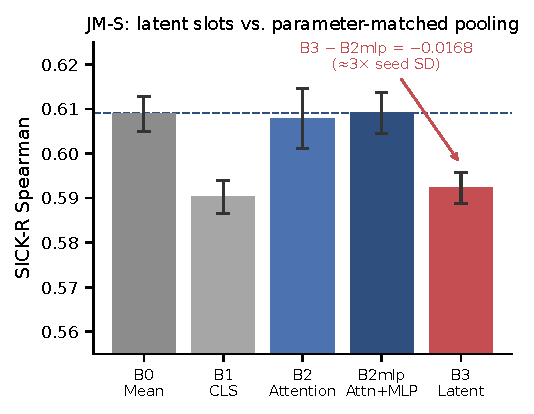
\includegraphics[width=\columnwidth]{figs/fig1_jms_sickr.pdf}
\caption{JM-S on SICK-R (mean $\pm$ SD over 3 seeds). The parameter-matched
attention control B2mlp (0.6091) exceeds the latent-slot arm B3 (0.5923) by
0.0168, roughly three seed standard deviations, in the direction opposite to
the success criterion.}
\label{fig:jms}
\end{figure}

\begin{table}[t]
\centering
\small
\caption{JM-S, SICK-R Spearman (3 seeds). The slot arm is last despite an equal
parameter budget; B2mlp is the fair comparator.}
\label{tab:jms}
\begin{tabular}{@{}llcc@{}}
\toprule
ID & Pooling & SICK-R & Params \\
\midrule
B0 & mean & $0.6089 \pm 0.0039$ & 291.87M \\
B1 & CLS & $0.5903 \pm 0.0037$ & 291.87M \\
B2 & attention & $0.6078 \pm 0.0067$ & 291.87M \\
B2mlp & attention + MLP & $\mathbf{0.6091 \pm 0.0045}$ & 292.92M \\
B3 & \textbf{latent slots} & $0.5923 \pm 0.0035$ & 292.92M \\
\bottomrule
\end{tabular}
\end{table}

\subsection{Result}

Table~\ref{tab:jms} and Figure~\ref{fig:jms} give the outcome:
$\mathrm{B3}-\mathrm{B2mlp} = -0.0168$ with a pooled seed SD of $0.0057$
($\approx3\sigma$). SciFact Recall@10 agrees in direction
(B0 0.0737, B2mlp 0.0678, B3 0.0619). Two independent holdouts therefore point
the same way.

\subsection{The obvious repair does not work}

Diagnostics showed the slots were not differentiated: pairwise slot-state
cosine $0.8716$ and attention-JS divergence $0.0437$ (near-uniform, i.e.\ all
slots read the same tokens). We therefore implemented the competitive
assignment mechanism of Slot Attention \cite{locatello2020} together with a
diversity loss, producing six repair arms (C1--C6).

\begin{figure}[t]
\centering
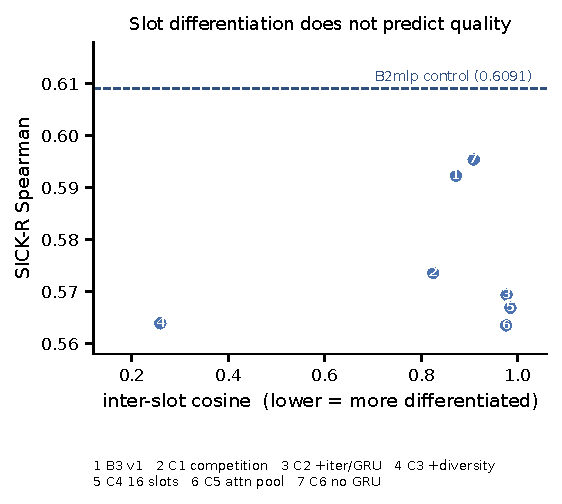
\includegraphics[width=\columnwidth]{figs/fig2_slot_diversity.pdf}
\caption{Slot differentiation versus quality. C3 (4) achieves the most
differentiated slots (cosine 0.259) yet the second-worst score; the best-
differentiated arms are not the best-performing ones. Differentiation is
therefore not the binding constraint.}
\label{fig:slots}
\end{figure}

The repairs succeed at their stated goal and fail at the real one
(Figure~\ref{fig:slots}). C1 raises attention JS from 0.044 to 0.089 and lowers
slot cosine from 0.872 to 0.825, i.e.\ the diagnosed symptom is fixed, and the
score drops to 0.5736. C3 drives slot cosine to \textbf{0.259} --- by every
structural measure the healthiest slot bank we produced --- and scores
$0.5639$, second worst. Multi-iteration refinement makes slots collapse faster
(C2 reaches cosine 0.977, and 0.998 before any training). Removing the GRU
gives the best repair (C6, 0.5954), still below B2mlp.

We read this as falsifying the ``slots failed because they did not
differentiate'' hypothesis. On short sentences (the SICK-R median is well under
128 tokens) attention pooling already covers every token, so additional slot
capacity has little to absorb. The original motivation for slots --- lossy
compression of long inputs --- is neither confirmed nor refuted by this task.

\section{JM-R: A Recurrent State That Cannot Help}
\label{sec:jmr}

\subsection{The one positive result, and why it is weak}

On a synthetic two-chunk task we constructed so that neither lexical overlap
nor single-chunk information can solve it (lexical ceiling 0.055--0.080 versus
chance 0.156; an oracle parser confirms 100\% derivability), the carried state
does help:

\begin{table}[t]
\centering
\small
\caption{Synthetic cross-chunk task, mean $\pm$ SD over 3 seeds (chance 0.167).
The fair \concat{} baseline removes the state's apparent advantage entirely.}
\label{tab:synth}
\begin{tabular}{@{}lc@{}}
\toprule
Arm & Accuracy \\
\midrule
\reset & $0.161 \pm 0.003$ \\
\shuffled & $0.162 \pm 0.018$ \\
\concat{} (unfair: embeddings summed) & $0.461 \pm 0.006$ \\
\concat{} (fair: joint encoding) & $0.491 \pm 0.007$ \\
\carried & $\mathbf{0.492 \pm 0.012}$ \\
\bottomrule
\end{tabular}
\end{table}

\begin{figure}[t]
\centering
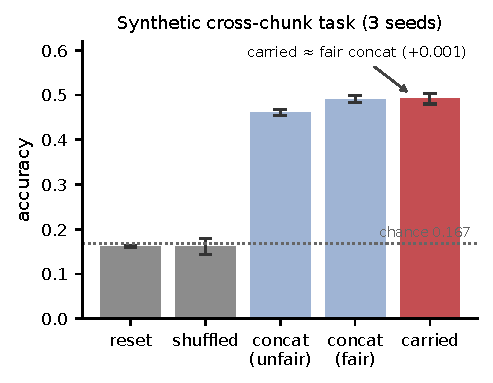
\includegraphics[width=\columnwidth]{figs/fig3_synthetic.pdf}
\caption{Synthetic task. \carried{} clears the no-memory controls by a wide
margin, but matches the fair \concat{} baseline to within 0.001, so the state
is a compression of information that joint encoding already exposes.}
\label{fig:synth}
\end{figure}

\carried{} beats \reset{} by $0.331$ (3/3 seeds, CI excludes 0) and \shuffled{}
behaves exactly like \reset{}, so the gain comes from correct content rather
than a generic bias. But the fair \concat{} baseline --- both chunks encoded
together, which is what an agent with sufficient context budget would do ---
scores $0.491$, statistically indistinguishable from \carried{} at $0.492$
(paired differences $+0.002$, $+0.010$, $-0.009$). Our earlier claim that
state transfer beat concatenation was an artifact of an unfair baseline in
which two independent embeddings were summed without a second forward pass.

\subsection{Real text: below the pre-registered bar}

On SciFact (three-stage abstract$\to$claim classification, 228 test claims,
document-component splits), \carried{} attains the highest mean Macro-F1
(Table~\ref{tab:scifact}), but the pre-registered criterion
(Eq.~\ref{eq:criterion}) is not met: \carried{} exceeds \shuffled{} in only
$2/3$ seeds, and the accuracy bootstrap CI contains zero for $2$ of $3$ seeds.

\begin{table}[t]
\centering
\small
\caption{SciFact transfer, Macro-F1 (constant-predictor baseline 0.196). The
mean ordering favors \carried{}, but the \shuffled{} contrast fails the
pre-registered sign test in one seed.}
\label{tab:scifact}
\begin{tabular}{@{}lc@{}}
\toprule
Condition & Macro-F1 \\
\midrule
\carried & $\mathbf{0.3151 \pm 0.0408}$ \\
\concat & $0.2953 \pm 0.0259$ \\
\shuffled & $0.2866 \pm 0.0193$ \\
\reset & $0.2553 \pm 0.0227$ \\
\bottomrule
\end{tabular}
\end{table}

\subsection{Nine pre-registered runs}

We fixed three paper-level splits and three seeds per split (9 runs) with a
frozen protocol specifying success criteria S1--S4 and forbidding any
adjustment. The outcome is uniformly negative
(Figure~\ref{fig:nine}): $\carried-\static = -0.0210$, 95\% CI
$[-0.0414, +0.0170]$, and \textbf{9/9 runs negative}. We report this despite
the CI containing zero because the sign consistency is itself informative.

\begin{figure}[t]
\centering
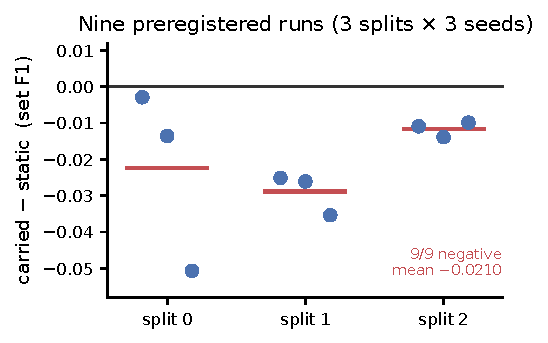
\includegraphics[width=\columnwidth]{figs/fig8_nine_runs.pdf}
\caption{Nine pre-registered runs. Every paired difference is negative; the red
bar is the per-split mean. Because training never left chance on this task
(\S\ref{sec:limits}), these runs \emph{cannot} adjudicate the mechanism --- we
report them as a bounded, protocol-respecting negative.}
\label{fig:nine}
\end{figure}

\subsection{Long documents: the state collapses}

On Qasper \citep{dasigi2021} (12 chunks, 93\% of test items have evidence at
distance $\ge8$),
the state pathway collapses outright: loss stays at $\ln 12 = 2.479$, block
representations become nearly identical (inter-block cosine 0.990, SD 0.0036),
and similarity rises monotonically with position rather than reflecting
content. State norm grows from 37.2 to 205.3 within 12 chunks.

\section{Diagnosing the State Pathway}
\label{sec:diag}

We localized the failure by measuring each stage in isolation
(Figure~\ref{fig:pathway}).

\begin{figure}[t]
\centering
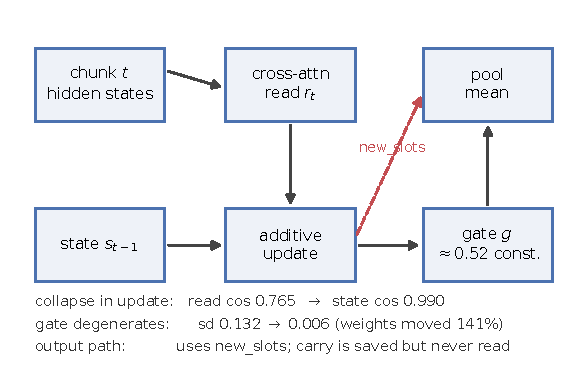
\includegraphics[width=\columnwidth]{figs/fig9_pathway.pdf}
\caption{The audited pathway. The dashed red edge is the one used for the
output; the carried state (via the gate) is stored but never read. Collapse
occurs in the additive update, and the gate converges to a constant.}
\label{fig:pathway}
\end{figure}

\paragraph{(i) The output never reads state.} Expanding
Eqs.~\eqref{eq:jmr}--\eqref{eq:jmr-out} for a single read iteration,
\begin{equation}
e^{(t)} = \mathrm{Norm}\Big(W_p\big[\mathrm{mean}(S^{(t-1)}) + \mathrm{mean}(R^{(t)})\big]\Big),
\end{equation}
so the previous state enters only as a \emph{task-independent additive term}
$\mathrm{mean}(S^{(t-1)})$, while all chunk-specific information comes from
$R^{(t)}$, which depends on chunk $t$ alone. We verified this empirically:
$\mathrm{mean}(S^{(t)})$ and the model's output are \emph{bit-identical}
($\max|\Delta| = 0$), and linear probes recover value information equally well
from either ($R^2 = 0.3847$ both), ruling out ``pooling discards slot
structure'' (best single slot $R^2 = 0.4149$, flattened slots $0.3342$,
inter-slot cosine 0.935).

\paragraph{(ii) The update dilutes new chunks.} Cross-attention read-outs
\emph{are} discriminative --- counterfactually swapping two chunks changes
$\|R\|$ by $0.0960$ --- but the additive update attenuates it $6.2\times$,
to $\|\Delta S\| = 0.0155$. The relative change decays monotonically with
chunk index (Figure~\ref{fig:decay}), from $0.318$ at chunk 1 to $0.098$ at
chunk 11, while consecutive-state cosine rises to $0.9992$. Gradients are not
the problem (backbone gradient norm 1298); large-batch contrastive training
would additionally require gradient caching \citep{gao2021}.

\begin{figure}[t]
\centering
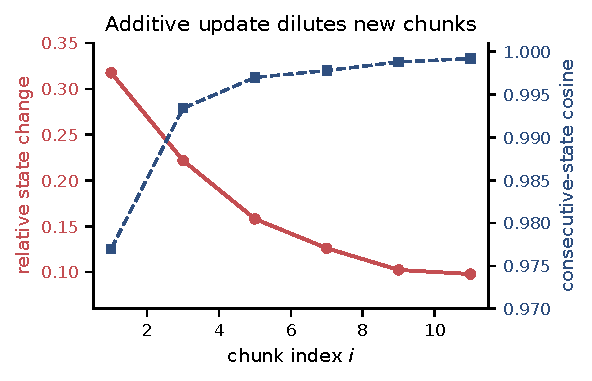
\includegraphics[width=\columnwidth]{figs/fig5_state_decay.pdf}
\caption{Additive update dilutes each new chunk. Relative state change
(left axis) decays monotonically; consecutive-state cosine (right axis)
approaches 1. Collapse originates in the update, not the read-out, whose
inter-block cosine is 0.765.}
\label{fig:decay}
\end{figure}

\paragraph{(iii) The gate degenerates, and it is trained to.} The gate
(Eq.~\ref{eq:gate}) starts with SD $0.1316$ under random inputs and ends after
one epoch with SD $0.0063$ --- a $21\times$ contraction to a near-constant
$g\approx0.52$. Its weights nevertheless move by 141\% relative to
initialization, so this is not an untrained module: the optimizer actively
converges on a solution that ignores its input.

\paragraph{(iv) The gate is not the constraint.} If the gate were the
bottleneck, forcing a better value should help. Freezing the checkpoint and
sweeping $g$ over $\{0.10,0.30,0.50,0.70,0.90,0.99\}$ yields accuracies
$0.082, 0.115, 0.066, 0.098, 0.090, 0.074$ --- no monotonic trend, and every
value inside chance $\pm2$SE (Figure~\ref{fig:gate}). Whatever is mixed, the
state holds nothing useful for the task.

\begin{figure}[t]
\centering
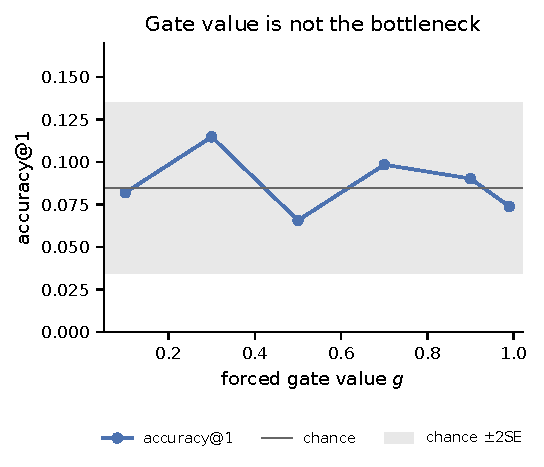
\includegraphics[width=\columnwidth]{figs/fig6_gate_sweep.pdf}
\caption{Forced gate sweep on a frozen checkpoint. All six values fall within
chance $\pm2$SE (shaded), and there is no trend. Gate value is not the
bottleneck.}
\label{fig:gate}
\end{figure}

\paragraph{Normalization fixes scale, not direction.} Two bounded update
variants (LayerNorm on $S{+}R$; gated bounded interpolation) bring state norm
from $205.3$ down to $64.0$ and lift validation accuracy from $0.049$ to
$0.123$, but inter-block cosine stays at $0.99$ --- they constrain magnitude
without restoring discriminability. Both still fail $\carried>\reset$.

\section{Methodological Findings}
\label{sec:method}

Each of the following had produced a wrong conclusion in our own pipeline
before it was corrected.

\paragraph{M1: Probes can be solvable without memory.} We added a lexical
ceiling: the accuracy attainable by bag-of-words matching against the final
chunk, with no model. Four of six probes are invalidated
(Figure~\ref{fig:probe}): ceilings are \textbf{1.00} (conflict), \textbf{0.63}
(isolation), \textbf{0.53} (order), and \textbf{0.23} (distractor), against
best model scores of 1.00, 0.43, 0.60, and 0.63. A probe is uninformative
whenever its ceiling meets or exceeds the model. The conflict probe's ceiling
of 1.00 means it can be solved perfectly without reading memory; one arm did
score 1.000 on it, which without the ceiling would have been reported as a
headline success. The probe required four redesigns, each refuted by a control,
and we report it as a cautionary case rather than a usable measurement.

\begin{figure}[t]
\centering
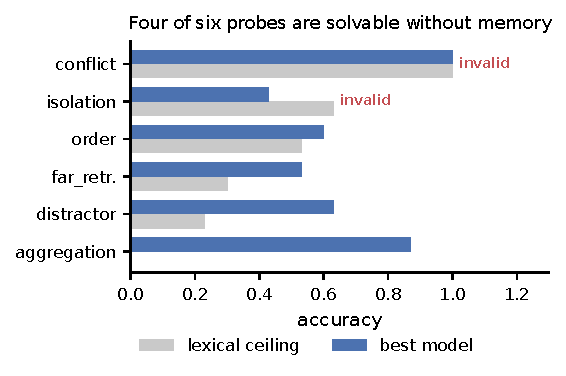
\includegraphics[width=\columnwidth]{figs/fig4_probe_validity.pdf}
\caption{Probe validity. Grey bars are lexical-overlap ceilings; blue bars are
the best model score. A probe is uninformative whenever the ceiling meets or
exceeds the model. Only \texttt{aggregation} is fully clean.}
\label{fig:probe}
\end{figure}

\paragraph{M2: Filtering before splitting leaks baseline performance.} An
earlier construction dropped samples on which BM25's top-1 was an evidence
block. The filter uses no labels but does use the baseline's behavior, turning
the test set into ``the samples where BM25 failed''. Removing it raised the
sample count from 592 to 881 and the BM25 test F1 from \textbf{0.140 to 0.302},
a $2.2\times$ underestimate.

\paragraph{M3: A missing projection made a working model look broken.} The
evaluator returned pre-projection pooled vectors while the model's embedding is
$\mathrm{project}\to\ell_2$. A model at 0.656 train accuracy measured 0.16
(below chance) and all arms became indistinguishable. When train performance
far exceeds evaluation, suspect the evaluator first.

\paragraph{M4: Full fine-tuning destroys a pretrained signal.} The Stage-1
encoder has block-level separation $\cos(\text{gold})-\cos(\text{other}) =
+0.021$ with no training (mean gold rank 3.42 of 6). Fine-tuning on 514
examples at $10^{-5}$, $3\times10^{-5}$, and $10^{-4}$ reduces separation to
$+0.0044$, $+0.0032$, and $0.0000$ respectively, while gradients remain
healthy (norm 14.3). A frozen backbone with a 524.8K-parameter head reaches
0.215 F1 in 170 seconds, beating 25 minutes of full fine-tuning. Small-data
fine-tuning of large encoders is over-parameterized fine-tuning
(Figure~\ref{fig:ft}).

\begin{figure}[t]
\centering
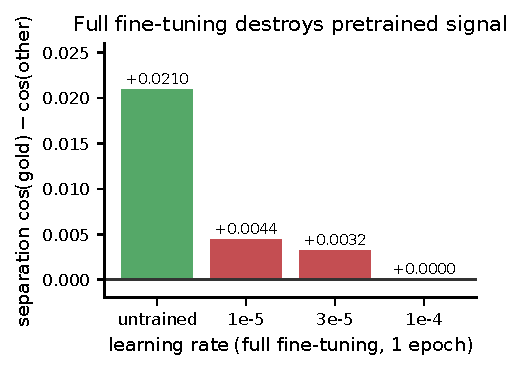
\includegraphics[width=0.88\columnwidth]{figs/fig7_finetune_sep.pdf}
\caption{Block-level separation before and after one epoch of full
fine-tuning. Every learning rate collapses the signal, confirming the effect
is not a tuning artifact.}
\label{fig:ft}
\end{figure}

\paragraph{M5: Small-sample positives vanish.} At $n{=}300$, \carried{}
appeared to beat both \reset{} and \concat{} for the first time in the study
($+0.050$). At $n{=}1500$ the effect collapsed to $+0.002$. Separately, a
``spread $>0.02$'' criterion claimed the gate mattered; replaced by a
monotonicity-and-$\pm2$SE test, the conclusion reversed. Directional agreement
across runs is not significance.

\section{Established Facts}

Measured directly, independent of interpretation: (1) the 350M encoder has
block-level signal with zero training (+0.021 separation; mean gold rank 3.42);
(2) full fine-tuning destroys it at every learning rate tested; (3) state is
worse than the chunk's own vector as a block representation
($-0.0785$, 5/5 runs); (4) state is order-sensitive (\carried{} above
\shuffled{} by $+0.0321$, 5/5), so it carries paper-level information;
(5) \textbf{the encoder's semantic representation is weaker than BM25} on this
task (0.28--0.31 versus 0.322, zero training); (6) slot differentiation does
not predict quality; (7) state norm diverges ($37.2\to205.3$) and inter-block
cosine approaches 1; (8) the gate degenerates to a constant despite 141\%
weight movement.

\section{What This Does and Does Not Show}

\paragraph{Supported.} In this implementation, latent slots add nothing over a
parameter-matched attention pooler, and a recurrent state is unsuitable as a
per-chunk representation while carrying only information that joint encoding
already provides.

\paragraph{Not supported.} That neural memory is impossible; that the state
channel can never work; that the designs are wrong \emph{in principle}. We
tested one pathway, one objective (NLI contrastive), one base checkpoint, and
one task family.

\paragraph{Why we stopped.} The pathology is structural (output path, update
rule, gate), three independent measurements agree, longer sequences worsen
rather than mitigate it, and every surface-level repair we tried
(differentiation, normalization, gate forcing) left the mechanism-layer test
failing. Continuing would require a different pathway, not more tuning.

\paragraph{The one untested question.} Every experiment here asks whether
state can \emph{carry} information. None asks whether a model can \emph{judge
what to remember} --- salience, importance, type. That requires no working
state channel and is the only direction this work does not refute.

\section{Limitations}
\label{sec:limits}

Test sets are small (168--179 per split; SciFact 228; probes 30). Only three
independent splits exist, with three seeds on one. Only one task family
(block-level evidence localization) and one base checkpoint were tested. BM25
was not trained as the model was, so the comparison is not
equal-condition. Most importantly, training used maximum length 128 while the
architecture declares 8192: \textbf{long-sequence capability was never truly
trained or tested}, so the compression regime that motivated latent slots
remains unexamined. Multilinguality is untested.

\section{Reproduction}

Code, per-run configs (seed, hyperparameters), summaries (steps, throughput,
peak memory), and evaluation JSON are released at
\url{https://modelscope.cn/models/LightNeko/Jaume} together with the frozen
pre-registration and figure-generation script. The full consolidated report is
in \texttt{docs/memory-report.md} (Chinese) and
\texttt{docs/memory-report.en.md} (English).

\begin{thebibliography}{9}

\bibitem{locatello2020}
F.~Locatello, D.~Weissenborn, T.~Unterthiner, A.~Mahendran, G.~Heigold,
J.~Uszkoreit, A.~Dosovitskiy, and M.~Kipf.
\newblock Object-centric learning with slot attention.
\newblock In \emph{NeurIPS}, 2020. arXiv:2006.15055.

\bibitem{reimers2019}
N.~Reimers and I.~Gurevych.
\newblock Sentence-BERT: Sentence embeddings using Siamese BERT-networks.
\newblock In \emph{EMNLP}, 2019.

\bibitem{gao2021}
L.~Gao, Y.~Zhang, J.~Han, and J.~Callan.
\newblock Scaling deep contrastive learning batch size under memory limited
setup.
\newblock arXiv:2101.06983, 2021.

\bibitem{thakur2021}
N.~Thakur, N.~Reimers, A.~R{\"u}ckl{\'e}, A.~Srivastava, and I.~Gurevych.
\newblock BEIR: A heterogeneous benchmark for zero-shot evaluation of
information retrieval models.
\newblock In \emph{NeurIPS Datasets and Benchmarks}, 2021.

\bibitem{dasigi2021}
A.~Dasigi, K.~Lo, I.~Beltagy, A.~Cohan, N.~A.~Smith, and M.~Gardner.
\newblock A dataset of information-seeking questions and answers anchored in
research papers.
\newblock In \emph{NAACL}, 2021.

\end{thebibliography}

\end{document}
